% =============================================================================
%  Rapport d'ingénierie des données — Projet 0 : Ubisoft vs Electronic Arts (FR)
%  Compilation : latexmk -xelatex rapport-fr.tex   (voir README.md de ce dossier)
% =============================================================================
\documentclass[11pt, a4paper, oneside, headings=normal, numbers=noenddot, DIV=12]{scrartcl}
\usepackage[french]{babel}
\usepackage{steam-report}
\graphicspath{{../livraison/figures/fr/}}
\sisetup{locale=FR, group-minimum-digits=4}

% --- Métadonnées ---------------------------------------------------------------
\newcommand{\ReportAuthor}{LUMU BAMANA MANASSE}
\newcommand{\ReportAuthorRole}{Data engineer}
\newcommand{\ReportShortTitle}{Ubisoft vs Electronic Arts · Rapport d'ingénierie des données}
\newcommand{\ReportFooter}{Octobre 2026 · v1.0.0}
\newcommand{\ReportKicker}{Rapport d'ingénierie des données · Projet 0}
\newcommand{\ReportTitle}{Ubisoft vs\\Electronic Arts}
\newcommand{\ReportSubtitle}{Ce que révèlent les données Steam :\\un pipeline ETL de bout en bout, du brief client à la recette}
\newcommand{\RepoURL}{https://github.com/MediJr/ubisoft-vs-ea-steam-etl}
\newcommand{\ReportMeta}{%
  \begin{tabularx}{\linewidth}{@{}>{\bfseries}l@{\hspace{1em}}Y@{}}
  Date & Octobre 2026 \\
  Version & 1.0.0 (livrée et recettée) \\
  Client & Lumen Forge Games (fictif) · Mission LFG-2026-001 \\
  Dépôt GitHub & \url{https://github.com/MediJr/ubisoft-vs-ea-steam-etl} \\
  Langue & Français · \textit{English version available in the repository}
  \end{tabularx}}
\newcommand{\ReportScenario}{Scénario fictif, données réelles : le client et ses interlocuteurs sont inventés pour simuler une mission
  professionnelle complète. Les données analysées proviennent des API publiques de Steam et de SteamSpy, extraites le 21 octobre 2026.
  Ce projet n'est affilié ni à Ubisoft, ni à Electronic Arts, ni à Valve.}
\hypersetup{pdftitle={Ubisoft vs Electronic Arts : rapport d'ingénierie des données}, pdfauthor={Lumu Bamana Manasse},
  pdfsubject={Pipeline ETL Steam, projet de portfolio}, pdflang={fr-FR}}

\begin{document}
\MakeTitlePage

% =============================================================================
\section*{Fiche du document}
\addcontentsline{toc}{section}{Fiche du document}

\begin{tabularx}{\linewidth}{@{}>{\bfseries\sffamily}L{4.2cm}Y@{}}
\toprule
Projet & Projet 0 du portfolio : pipeline ETL sur les données publiques de Steam \\
Mission & LFG-2026-001 : « Comprendre ce qui fonctionne chez les grands éditeurs sur Steam » \\
Client & Lumen Forge Games, studio indépendant lyonnais (fictif), à l'attention de Camille Roux \\
Auteur & Lumu Bamana Manasse, data engineer \\
Période de réalisation & Octobre 2026 \\
Données & Extraction du 21 octobre 2026, de 18 h 38 à 19 h 10 (heure de Paris) \\
Statut & \pill{good}{LIVRÉ} \pill{good}{RECETTÉ AVEC RÉSERVES MINEURES} \\
Code source & \url{https://github.com/MediJr/ubisoft-vs-ea-steam-etl} \\
\bottomrule
\end{tabularx}

\subsection*{Historique des versions}
\begin{tabularx}{\linewidth}{@{}l l Y@{}}
\toprule
\textbf{Version} & \textbf{Date} & \textbf{Objet} \\
\midrule
0.1 & 21/10/2026 & Cadrage : brief, compte rendu, cahier des charges \\
0.9 & 21/10/2026 & Pipeline complet, analyses, corrections de qualité des données \\
1.0.0 & 22/10/2026 & Recette, rapport final (français et anglais), publication \\
\bottomrule
\end{tabularx}

\subsection*{Guide de lecture}
\begin{tabularx}{\linewidth}{@{}>{\bfseries}L{4.2cm}Y@{}}
Décideur (client) & \hyperref[sec:resume]{1. Résumé exécutif} et \hyperref[sec:resultats]{11. Résultats et recommandations} \\
Responsable data & 2. Cadrage, 4. Architecture, 7. Qualité, 10. Recette, 12. Limites \\
Ingénieur reprenant le projet & 5. Pipeline, 6. Modèle de données, 9. Exploitation, annexes \\
\end{tabularx}

\begingroup
\addtokomafont{sectionentry}{\color{primary}}
\setcounter{tocdepth}{2}
\tableofcontents
\endgroup
\clearpage

% =============================================================================
\section{Résumé exécutif}\label{sec:resume}

\textbf{Le besoin.} Lumen Forge Games, un studio indépendant sans équipe data, prépare la sortie de son premier jeu sur Steam
à environ 25~€. Avant de fixer son prix et sa stratégie de lancement, il veut savoir ce qui fonctionne
(et ce qui échoue) chez deux grands éditeurs : \textbf{Ubisoft} et \textbf{Electronic Arts}.

\textbf{La solution.} Un pipeline ETL en Python collecte automatiquement les données publiques de Steam et de SteamSpy
(six sources), les nettoie, puis les charge dans une base analytique DuckDB. Dix requêtes SQL répondent aux quatre
questions business, et un rapport présente les résultats. Le tout s'exécute en \textbf{une seule commande}.

\kpirow{100}{jeux analysés\\(50 par éditeur)}{9,8 M}{avis Steam\\agrégés}{930}{réponses d'API\\brutes conservées}{0}{donnée personnelle\\collectée}
\kpirow{6}{sources de\\données}{30 min}{extraction complète\\(clone neuf)}{2 s}{rejeu d'un lot\\sans appel d'API}{6 / 6}{critères de recette\\conformes}

\begin{keybox}[Principaux résultats]
\begin{itemize}[leftmargin=1.2em]
  \item \textbf{Q1 · Satisfaction :} égalité en moyenne (80~\%), mais deux profils opposés. EA joue « quitte ou double »
        (médiane de 85~\%, mais 11 jeux sous 70~\%). Ubisoft est plus régulier, et ses jeux \textbf{gagnent 3,2 points après leur sortie}.
  \item \textbf{Q2 · Prix :} plus un jeu est cher, moins il est bien noté (corrélation d'environ $-0{,}5$). Au-delà de 60~€, la satisfaction chute.
  \item \textbf{Q3 · Longévité :} les jeux qui durent sont gratuits ou multijoueurs.
  \item \textbf{Q4 · Francophones :} légèrement plus généreux (+2 points), mais ils ne rédigent que 2~\% des avis.
\end{itemize}
\end{keybox}

\textbf{Ce que démontre ce projet, côté ingénierie :} une extraction respectueuse des API (pauses, réessais, cache de reprise),
une couche brute immuable et datée, un chargement transactionnel sans doublon, la protection des données \emph{dès la conception}
(aucun pseudo de joueur n'est jamais téléchargé), la détection et la correction de quatre problèmes de qualité dans des données réelles,
et une reprise après incident documentée.

% =============================================================================
\section{Contexte et cadrage}

\subsection{De la demande floue aux questions mesurables}
La demande initiale tenait en une phrase : « comprendre ce qui marche chez les gros éditeurs ». La réunion de cadrage l'a transformée
en quatre questions, chacune liée à une décision concrète du client.

\begin{table}[H]
\centering
\begin{tabularx}{\linewidth}{@{}l Y L{4.1cm}@{}}
\toprule
\textbf{\#} & \textbf{Question business} & \textbf{Décision éclairée} \\
\midrule
Q1 & Lequel des deux éditeurs satisfait le mieux ses joueurs sur Steam, et cette satisfaction est-elle stable dans le temps ? & Suivi de réputation après la sortie \\
Q2 & Un jeu plus cher est-il mieux noté ? Les promotions sont-elles un signe de difficulté ? & Prix de lancement et promotions \\
Q3 & Quels jeux gardent leurs joueurs des années après leur sortie ? & Contenu après le lancement \\
Q4 & Les joueurs francophones jugent-ils différemment ces éditeurs ? & Marché prioritaire \\
\bottomrule
\end{tabularx}
\caption{Questions business retenues lors du cadrage}
\end{table}

\subsection{Périmètre}
\begin{tabularx}{\linewidth}{@{}Y Y@{}}
\toprule
\textcolor{good}{\textbf{Inclus}} & \textcolor{warn}{\textbf{Exclu}} \\
\midrule
Jeux de type \texttt{game} publiés sur Steam par Ubisoft ou EA & DLC, bandes-son, démos, éditions groupées \\
Au moins 500 avis, 50 jeux maximum par éditeur (les plus commentés) & Autres plateformes : EA app, Ubisoft Connect, consoles \\
Fiches, synthèses d'avis, historique mensuel, fréquentation & Texte des avis et toute donnée personnelle \\
Rapport d'analyse et pipeline relançable & Impact boursier, tableau de bord interactif, planification automatique \\
\bottomrule
\end{tabularx}

\subsection{Démarche}
Le projet suit les cinq phases d'une mission de conseil en données. Chaque phase produit des livrables versionnés dans le dépôt.

\begin{table}[H]
\centering\small
\begin{tabularx}{\linewidth}{@{}l L{3.2cm} Y@{}}
\toprule
\textbf{Phase} & \textbf{Objet} & \textbf{Livrables} \\
\midrule
1 & Cadrage & Brief client, compte rendu de cadrage, cahier des charges (\texttt{docs/mission/}) \\
2 & Extraction & \texttt{src/extract.py}, couche brute \texttt{data/raw/}, ADR 002 \\
3 & Transformation et chargement & \texttt{src/transform.py}, \texttt{src/load.py}, \texttt{sql/00\_schema.sql} \\
4 & Analyse & 10 requêtes SQL, 5 graphiques, résultats générés automatiquement \\
5 & Livraison & Recette (PV), présent rapport, documentation, publication \\
\bottomrule
\end{tabularx}
\caption{Phases de la mission}
\end{table}

% =============================================================================
\section{Sources de données}

\begin{table}[H]
\centering\small
\begin{tabularx}{\linewidth}{@{}L{3.8cm} L{2.0cm} Y L{1.9cm}@{}}
\toprule
\textbf{Source} & \textbf{Statut} & \textbf{Données utilisées} & \textbf{Usage} \\
\midrule
Recherche Steam Store & Non officiel & Liste des jeux d'un éditeur (identifiants \texttt{app\_id}) & Périmètre \\
Fiche Steam (\texttt{appdetails}) & Public, non documenté & Éditeur, prix en euros, remise, genres, date de sortie & Q2, Q3 \\
Avis (\texttt{appreviews}) & Public, documenté & Totaux d'avis, toutes langues et en français & Q1, Q4 \\
Historique (\texttt{appreviewhistogram}) & Non officiel & Avis positifs et négatifs par mois & Q1 \\
Steam Web API & Officiel & Joueurs connectés & Q3 \\
SteamSpy & Tiers & Estimation des possesseurs, pic de la veille & Information \\
\bottomrule
\end{tabularx}
\caption{Inventaire des sources}
\end{table}

\textbf{Contraintes.} Steam tolère environ 200 requêtes par tranche de 5 minutes. Trois points d'accès ne sont pas officiels et peuvent
changer sans préavis. Aucune clé d'API n'est requise, donc il n'y a aucun secret à gérer.

\begin{keybox}[Exploration préalable : tester avant de s'engager]
Avant de signer le cahier des charges, chaque point d'accès a été testé à la main. Le paramètre \texttt{day\_range} de l'API des avis
\emph{semble} filtrer les avis sur une période, mais en réalité il \textbf{ne modifie pas} la synthèse renvoyée. Sans ce test, la mesure
de stabilité (Q1) aurait été promise sur une base fausse. C'est l'historique mensuel (\texttt{appreviewhistogram}) qui l'a rendue possible.
\end{keybox}

% =============================================================================
\section{Architecture de la solution}

\begin{figure}[H]
\centering
\resizebox{\linewidth}{!}{%
\begin{tikzpicture}[
  font=\sffamily\small, node distance=0.5cm and 0.9cm,
  src/.style={draw=rule, fill=panel, rounded corners=2pt, minimum width=2.7cm, minimum height=0.75cm, align=center},
  stage/.style={draw=primary, fill=primary, text=white, rounded corners=3pt, minimum width=2.5cm, minimum height=1.3cm, align=center, font=\sffamily\small\bfseries},
  store/.style={cylinder, shape border rotate=90, aspect=0.18, draw=accent, fill=accent!8, minimum width=2.3cm, minimum height=1.5cm, align=center},
  deliv/.style={draw=accent, rounded corners=2pt, minimum width=2.6cm, minimum height=0.75cm, align=center},
  arr/.style={-{Stealth[length=2.6mm]}, thick, color=ink2}]
  \node[src] (s1) {Steam Store\\\scriptsize recherche + fiches};
  \node[src, below=of s1] (s2) {Avis Steam\\\scriptsize synthèse + historique};
  \node[src, below=of s2] (s3) {Steam Web API\\\scriptsize joueurs connectés};
  \node[src, below=of s3] (s4) {SteamSpy\\\scriptsize estimations};
  \node[stage, right=1.2cm of $(s2.east)!0.5!(s3.east)$] (e) {EXTRACT\\\scriptsize\mdseries 2 passes · cache};
  \node[store, below=1.1cm of e] (raw) {\scriptsize data/raw/\\\scriptsize AAAA-MM-JJ\\\scriptsize JSON + manifeste};
  \node[stage, right=of e] (t) {TRANSFORM\\\scriptsize\mdseries périmètre · typage};
  \node[stage, right=of t] (l) {LOAD\\\scriptsize\mdseries transaction};
  \node[store, right=of l] (db) {\scriptsize DuckDB\\\scriptsize 5 tables};
  \node[deliv, right=1.1cm of db, yshift=1.1cm] (o1) {10 requêtes SQL};
  \node[deliv, below=0.35cm of o1] (o2) {5 graphiques};
  \node[deliv, below=0.35cm of o2] (o3) {Rapport + recette};
  \foreach \s in {s1,s2,s3,s4} \draw[arr] (\s.east) -- (e.west);
  \draw[arr] (e) -- node[right, font=\scriptsize\sffamily, text=ink2]{écrit tel quel} (raw);
  \draw[arr] (raw.east) -| (t.south);
  \draw[arr] (t) -- (l);
  \draw[arr] (l) -- (db);
  \foreach \o in {o1,o2,o3} \draw[arr] (db.east) -- (\o.west);
  \begin{scope}[on background layer]
    \node[draw=rule, dashed, rounded corners=6pt, fit=(e)(t)(l)(raw), inner sep=10pt, label={[font=\scriptsize\sffamily, text=ink2]above:python -m src.pipeline}] {};
  \end{scope}
\end{tikzpicture}}
\caption{Architecture du pipeline : une commande enchaîne extraction, transformation, chargement et production du rapport}
\end{figure}

\subsection{Choix techniques}
\begin{table}[H]
\centering\small
\begin{tabularx}{\linewidth}{@{}L{2.5cm} L{3.4cm} Y@{}}
\toprule
\textbf{Besoin} & \textbf{Choix} & \textbf{Justification et alternatives écartées} \\
\midrule
Langage & Python 3.14 & Standard du data engineering, écosystème riche \\
Appels HTTP & \texttt{requests} & Simple et fiable. \texttt{httpx} (asynchrone) est inutile à ce volume. \\
Transformation & \texttt{pandas} & Adapté à quelques milliers de lignes. Polars est plus rapide, mais sans gain ici. \\
Stockage & DuckDB (fichier) & SQL analytique sans serveur. PostgreSQL sera la nouveauté du projet 1. \\
Analyse & SQL & Lisible, vérifiable, indépendant de Python \\
Graphiques & \texttt{matplotlib} & Figures statiques intégrables au rapport \\
Environnement & \texttt{venv} + \texttt{pip} & Universel. \texttt{uv} et Poetry seront introduits plus tard. \\
Orchestration & Aucune (une commande) & Volontaire au niveau 0. Dagster est prévu au projet 3. \\
\bottomrule
\end{tabularx}
\caption{Stack technique (détail : ADR 001)}
\end{table}

\subsection{Principes de conception}
\begin{enumerate}[leftmargin=1.4em]
  \item \textbf{Couche brute immuable :} les réponses des API sont stockées sans modification. Un bug de transformation se corrige en
        rejouant le lot, sans réinterroger les API.
  \item \textbf{Idempotence :} exécuter deux fois le pipeline donne le même résultat, sans doublon (clés primaires, rechargement complet).
  \item \textbf{Protection des données dès la conception :} la donnée personnelle n'est jamais demandée aux API.
  \item \textbf{Reproductibilité :} chaque chiffre du rapport provient d'une requête versionnée. Le fichier \texttt{resultats.md} est régénéré à chaque exécution.
  \item \textbf{Traçabilité :} un manifeste par lot, une table des exclusions motivées, et trois ADR pour les décisions structurantes.
\end{enumerate}

% =============================================================================
\section{Conception du pipeline}

\subsection{Extraction}
Collecter les six sources pour les 160 jeux candidats aurait demandé environ 1\,000 appels, soit plus de 25 minutes,
pour des jeux dont une partie serait de toute façon écartée. L'extraction se fait donc en \textbf{deux passes} :

\begin{table}[H]
\centering\small
\begin{tabularx}{\linewidth}{@{}l Y r r@{}}
\toprule
\textbf{Étape} & \textbf{Action} & \textbf{Ubisoft} & \textbf{EA} \\
\midrule
Découverte & Recherche Steam par éditeur, catégorie « jeux » & 80 & 80 \\
Passe légère & Synthèse des avis (1 appel par jeu), filtre « au moins 500 avis » & 77 & 76 \\
Passe détaillée & 5 appels par jeu retenu & 77 & 76 \\
\bottomrule
\end{tabularx}
\caption{Entonnoir d'extraction (lot du 21/10/2026)}
\end{table}

\textbf{Robustesse.} Une pause de 1,5~s précède chaque appel. Les erreurs 429 (trop de requêtes) et 5xx déclenchent jusqu'à trois réessais
à délai croissant. Un \texttt{User-Agent} explicite identifie le projet. Chaque réponse est mise en cache dans la couche brute : une
extraction interrompue reprend là où elle s'est arrêtée. L'écriture est \textbf{atomique}, ajoutée après l'incident décrit en section~\ref{sec:incident} :

\begin{lstlisting}[language=Python]
temporary = path.with_suffix(".tmp")
temporary.write_text(json.dumps(payload, ensure_ascii=False, indent=2), encoding="utf-8")
temporary.replace(path)   # renommage instantané : jamais de fichier à moitié écrit
\end{lstlisting}

\textbf{Protection des données dès la source.} Les avis sont demandés avec \texttt{num\_per\_page=0} : Steam ne renvoie que des totaux,
sans aucun avis individuel, donc sans pseudo ni identifiant.

\subsection{Transformation}
\begin{table}[H]
\centering\small
\begin{tabularx}{\linewidth}{@{}L{3.4cm} Y@{}}
\toprule
\textbf{Règle} & \textbf{Mise en œuvre} \\
\midrule
Périmètre & Type \texttt{game}, déjà sorti, éditeur réel conforme à l'éditeur recherché \\
Plafond & Les 50 jeux les plus commentés de chaque éditeur. Les autres sont tracés dans \texttt{exclusions} (53 jeux). \\
Typage & Dates françaises (« 12 janv. 2023 ») converties en \texttt{DATE}, prix en euros, fourchettes SteamSpy en entiers \\
Valeurs manquantes & Taux d'avis \texttt{NULL} plutôt que 0 en l'absence d'avis. Un jeu gratuit vaut 0~€. \\
Historique & Horodatages Unix convertis en mois, agrégés si Steam renvoie un découpage hebdomadaire \\
\bottomrule
\end{tabularx}
\caption{Règles de transformation}
\end{table}

\subsection{Chargement}
Le chargement suit une stratégie de \textbf{rechargement complet} : le schéma est recréé, puis toutes les tables sont insérées,
\textbf{dans une seule transaction}. En cas d'échec, rien n'est validé et la base garde son état précédent. Elle n'est jamais à moitié chargée.

\begin{lstlisting}[language=Python]
connection.execute("BEGIN TRANSACTION")
try:
    connection.execute(SCHEMA_PATH.read_text(encoding="utf-8"))
    for name in LOAD_ORDER:                      # games d'abord (clés étrangères)
        connection.register("incoming", tables[name])
        connection.execute(f"INSERT INTO {name} BY NAME SELECT * FROM incoming")
        connection.unregister("incoming")
    connection.execute("COMMIT")
except Exception:
    connection.execute("ROLLBACK")
    raise
\end{lstlisting}

% =============================================================================
\section{Modèle de données}

\begin{figure}[H]
\centering
\resizebox{0.95\linewidth}{!}{%
\begin{tikzpicture}[font=\sffamily\scriptsize,
  ent/.style={draw=primary, fill=white, rounded corners=2pt, align=left, inner sep=5pt},
  rel/.style={-{Stealth[length=2mm]}, thick, color=accent}]
  \node[ent] (g) {\textbf{\normalsize games}\\[2pt]\textbf{app\_id} \textit{PK}\\name, publisher\_group\\price\_initial\_eur, discount\_percent\\steam\_release\_date, years\_on\_steam\\genres, metacritic\_score, \dots};
  \node[ent, left=1.6cm of g] (r) {\textbf{\normalsize review\_summary}\\[2pt]\textbf{app\_id, language} \textit{PK}\\total\_reviews, total\_positive\\positive\_rate};
  \node[ent, right=1.6cm of g] (m) {\textbf{\normalsize reviews\_monthly}\\[2pt]\textbf{app\_id, month} \textit{PK}\\reviews\_up, reviews\_down};
  \node[ent, below=1.2cm of g] (p) {\textbf{\normalsize player\_snapshot}\\[2pt]\textbf{app\_id, snapshot\_date} \textit{PK}\\current\_players\\peak\_players\_yesterday};
  \node[ent, dashed, draw=ink2, right=1.6cm of p] (x) {\textbf{\normalsize exclusions}\\[2pt]\textbf{app\_id, publisher\_searched} \textit{PK}\\reason};
  \draw[rel] (r) -- node[above]{2 par jeu} (g);
  \draw[rel] (m) -- node[above]{1 par mois} (g);
  \draw[rel] (p) -- node[right]{1 par jour} (g);
\end{tikzpicture}}
\caption{Modèle de données DuckDB (les flèches représentent les clés étrangères)}
\end{figure}

\begin{table}[H]
\centering\small
\begin{tabularx}{\linewidth}{@{}l Y r@{}}
\toprule
\textbf{Table} & \textbf{Grain (une ligne par…)} & \textbf{Lignes} \\
\midrule
\texttt{games} & jeu retenu & 100 \\
\texttt{review\_summary} & jeu et langue (\texttt{all}, \texttt{french}) & 200 \\
\texttt{reviews\_monthly} & jeu et mois & \num{9929} \\
\texttt{player\_snapshot} & jeu et date d'extraction & 100 \\
\texttt{exclusions} & jeu candidat écarté, avec son motif & 53 \\
\bottomrule
\end{tabularx}
\caption{Tables, grain et volumétrie (dictionnaire complet en annexe~\ref{ann:dico})}
\end{table}

% =============================================================================
\section{Qualité des données}

\subsection{Contrôles intégrés}
\begin{itemize}[leftmargin=1.2em]
  \item \textbf{Contraintes du schéma :} clés primaires, \texttt{NOT NULL}, clés étrangères. Une anomalie fait échouer le chargement au lieu de fausser les résultats.
  \item \textbf{Requête de contrôle} (\texttt{sql/controle\_recette.sql}) : absence de doublons, volume par éditeur, seuil d'avis, absence de colonne personnelle.
  \item \textbf{Table des exclusions :} chaque candidat écarté a un motif. Rien ne disparaît sans trace.
\end{itemize}

\subsection{Anomalies détectées et corrigées}
Les données réelles ont révélé quatre problèmes que la seule lecture de la documentation des API ne laissait pas prévoir.

\begin{table}[H]
\centering\small
\begin{tabularx}{\linewidth}{@{}L{3.1cm} Y Y@{}}
\toprule
\textbf{Symptôme} & \textbf{Cause} & \textbf{Correction} \\
\midrule
5 dates de sortie non reconnues & Steam écrit « aout » sans accent, et une fiche n'a aucune date & Dictionnaire des mois accepte les deux graphies. La date absente reste \texttt{NULL}. \\
\midrule
0 exclusion au premier passage : un résultat trop parfait & Les jeux écartés par le plafond de 50 n'étaient pas tracés & 53 exclusions motivées enregistrées \\
\midrule
Pic de joueurs à 0 pour 9 jeux récents (\textit{Battlefield 6} : 0, contre 45\,100 connectés) & SteamSpy ne suit pas encore ces jeux : 0 signifie « inconnu » & Bascule sur l'API officielle de Steam (ADR 003) \\
\midrule
« Lancement » de 21 jeux EA en 2020 & Retour d'EA sur Steam en 2020, et avis plus récents que certains jeux & Q1b exige des premiers avis contemporains de la sortie sur Steam \\
\bottomrule
\end{tabularx}
\caption{Problèmes de qualité rencontrés sur les données réelles}
\end{table}

\begin{keybox}[Leçon]
Un zéro n'est pas toujours un zéro, et un résultat parfait est suspect. La qualité des données ne se décrète pas : elle se vérifie,
jeu par jeu, avant toute analyse.
\end{keybox}

% =============================================================================
\section{Sécurité, conformité et gouvernance}

\begin{tabularx}{\linewidth}{@{}L{3.6cm} Y@{}}
\toprule
\textbf{Thème} & \textbf{Mesure} \\
\midrule
Données personnelles (RGPD) & L'API des avis peut renvoyer pseudos, identifiants et textes. En application de la \textbf{minimisation} (art.~5.1.c)
et de la \textbf{protection dès la conception} (art.~25), seuls des totaux sont demandés. Vérification : aucun champ \texttt{steamid} ni
\texttt{personaname} dans les 930 fichiers bruts, et aucune colonne personnelle dans la base. \\
Secrets & Aucune clé d'API requise. Le \texttt{.gitignore} exclut néanmoins tout fichier \texttt{.env}. \\
Données publiées & Les données ne sont pas versionnées (\texttt{data/} est ignoré) : elles se régénèrent avec le pipeline. \\
Usage des API & Débit limité volontairement, \texttt{User-Agent} explicite, usage non commercial \\
Traçabilité & Manifeste par lot, journal de bord daté, ADR, CHANGELOG \\
\bottomrule
\end{tabularx}

% =============================================================================
\section{Exploitation}

\subsection{Commandes}
\begin{lstlisting}[language=bash]
python -m venv .venv && .venv\Scripts\activate     # environnement isolé (Windows)
pip install -r requirements.txt
python -m src.pipeline                             # extraction du jour + traitement (~30 min)
python -m src.pipeline --run-date 2026-10-21       # rejeu d'un lot brut, sans appel d'API (~2 s)
\end{lstlisting}

\subsection{Capture d'une exécution complète}
Journal réel de la recette sur un environnement neuf (horodatages et chemins abrégés, progression intermédiaire masquée) :

\begin{terminal}{PowerShell · python -m src.pipeline}
\begin{lstlisting}[style=terminal]
19:16:24 | INFO | src.extract   | Extraction vers ...\00-jeux-video-etl\data\raw\2026-10-21
19:16:29 | INFO | src.extract   | Ubisoft : 80 jeux candidats
19:19:17 | INFO | src.extract   | Ubisoft : 76 jeux avec au moins 500 avis
19:31:55 | INFO | src.extract   | Electronic Arts : 80 jeux candidats
19:34:39 | INFO | src.extract   | Electronic Arts : 76 jeux avec au moins 500 avis
19:46:47 | INFO | src.extract   | Extraction terminée
19:46:47 | INFO | src.transform | Table games            :    100 lignes
19:46:47 | INFO | src.transform | Table review_summary   :    200 lignes
19:46:47 | INFO | src.transform | Table reviews_monthly  :   9768 lignes
19:46:47 | INFO | src.transform | Table player_snapshot  :    100 lignes
19:46:47 | INFO | src.transform | Table exclusions       :     52 lignes
19:46:47 | INFO | src.load      | Base chargée : ...\data\steam.duckdb
19:46:49 | INFO | src.report    | Graphiques et résultats écrits dans ...\docs\livraison
19:46:49 | INFO | pipeline      | Pipeline terminé en 1825 s
\end{lstlisting}
\end{terminal}

\subsection{Incident et reprise}\label{sec:incident}
\begin{table}[H]
\centering\small
\begin{tabularx}{\linewidth}{@{}l Y@{}}
\toprule
\textbf{Heure} & \textbf{Événement} \\
\midrule
18~h~38 & Lancement de l'extraction de production \\
19~h~05 & \textbf{Interruption externe} du processus, à 56 jeux EA sur 76 \\
19~h~06 & Diagnostic : aucun processus actif, aucun manifeste, 133 jeux en cache. Vérification : aucun fichier JSON tronqué. \\
19~h~06 & Relance de la même commande : les 133 jeux en cache sont relus en \textbf{0,1 s}, puis la collecte reprend \\
19~h~10 & Extraction terminée. Amélioration : écriture atomique, pour qu'un arrêt brutal ne laisse jamais de fichier corrompu. \\
\bottomrule
\end{tabularx}
\caption{Chronologie de l'incident du 21/10/2026}
\end{table}

% =============================================================================
\section{Tests et recette}

La recette a été menée sur un \textbf{environnement neuf} : copie des seuls fichiers publiables (38 fichiers, sans données ni
environnement virtuel), nouvel environnement Python, puis la commande unique du README.

\begin{table}[H]
\centering\small
\begin{tabularx}{\linewidth}{@{}l L{4.2cm} Y c@{}}
\toprule
\textbf{\#} & \textbf{Critère} & \textbf{Résultat} & \\
\midrule
C1 & Exécution de bout en bout en une commande & Installation en 54~s, pipeline en 30~min~25~s, code de retour 0 & \ok \\
C2 & Aucun doublon après une nouvelle exécution & Volumes identiques avant et après : 100 / 200 / \num{9929} / 100 / 53 & \ok \\
C3 & Au moins 15 jeux par éditeur & 50 jeux par éditeur, tous avec au moins 500 avis (minimum : \num{7215}) & \ok \\
C4 & Une requête et une réponse par question & 10 requêtes, une section par question & \ok \\
C5 & Aucune donnée personnelle & Aucun champ personnel dans 930 fichiers bruts ni dans la base & \ok \\
C6 & Limites explicitées & Section~\ref{sec:limites} & \ok \\
\bottomrule
\end{tabularx}
\caption{Résultats de la recette (détails : \texttt{docs/livraison/2026-10-21-pv-recette.md})}
\end{table}

\begin{warnbox}[Réserves mineures]
\textbf{R1 · Reproductibilité du panel.} L'ordre de pertinence de la recherche Steam varie légèrement d'une exécution à l'autre.
Entre la production et la recette, 99 jeux sur 100 sont identiques. Les indicateurs clés le sont au dixième près
(taux pondérés : EA 77,4~\%, Ubisoft 81,3~\%). \\
\textbf{R2 · Promotions.} Aucun jeu n'était en promotion le jour de l'extraction : cette partie de Q2 ne peut pas être tranchée.
\end{warnbox}

% =============================================================================
\section{Résultats et recommandations}\label{sec:resultats}

\subsection{Q1 · Qui satisfait le mieux ses joueurs, et durablement ?}
\begin{figure}[H]
\centering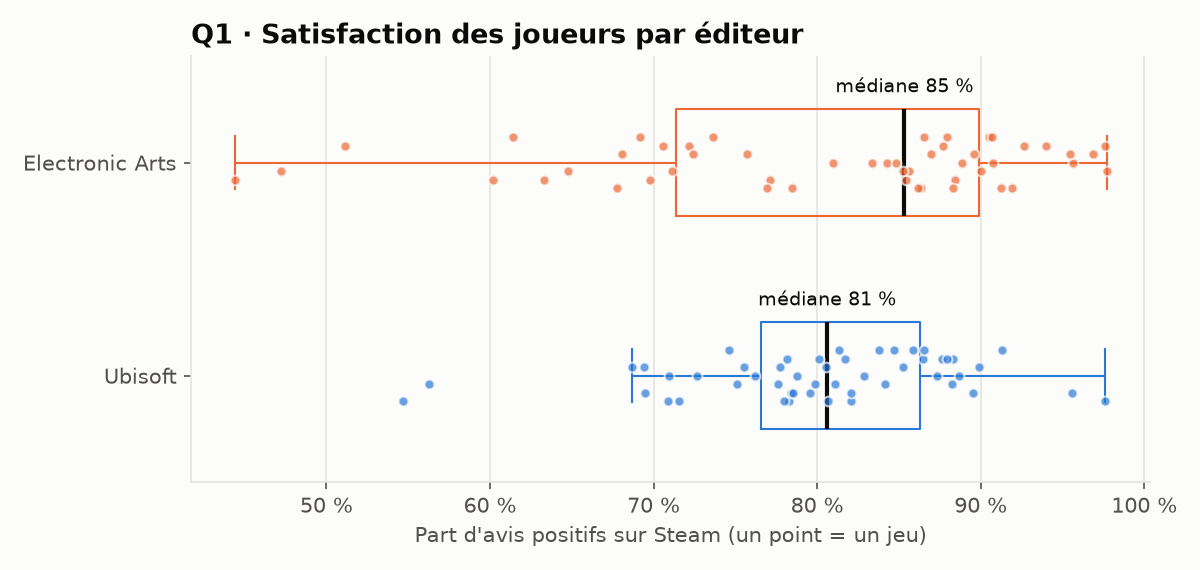
\includegraphics[width=0.92\linewidth]{q1_satisfaction_par_editeur.png}
\caption{Part d'avis positifs par jeu et par éditeur}
\end{figure}

\begin{table}[H]
\centering\small
\begin{tabularx}{\linewidth}{@{}Y r r r r r r@{}}
\toprule
\textbf{Éditeur} & \textbf{Moyenne} & \textbf{Médiane} & \textbf{Pondéré} & \textbf{< 70 \%} & \textbf{Évolution} & \textbf{Redressés} \\
\midrule
\textbf{Electronic Arts} & 80,3~\% & 85,3~\% & 77,4~\% & 11 & $-1{,}0$ pt & 4 / 34 \\
\textbf{Ubisoft} & 80,2~\% & 80,6~\% & 81,3~\% & 5 & $+3{,}2$ pts & 12 / 39 \\
\bottomrule
\end{tabularx}
\caption{Satisfaction globale, puis évolution entre les 3 premiers mois et les 12 derniers mois sur Steam}
\end{table}

Égalité en moyenne, mais deux profils : EA est plus dispersé (meilleure médiane, mais deux fois plus de jeux sous 70~\%), tandis
qu'Ubisoft est plus régulier et \textbf{améliore ses jeux après leur sortie} (\textit{Assassin's Creed Unity} +24,5 points,
\textit{The Crew 2} +25,5).

\begin{figure}[H]
\centering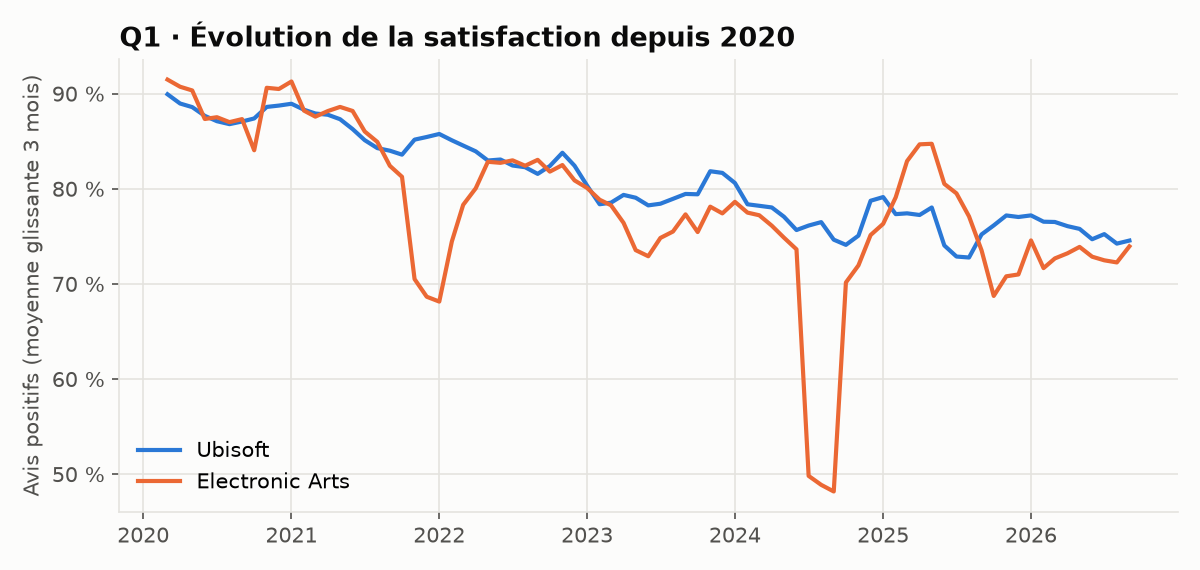
\includegraphics[width=0.92\linewidth]{q1_evolution_mensuelle.png}
\caption{Évolution mensuelle : deux crises visibles chez EA}
\end{figure}

L'historique mensuel révèle deux crises chez EA : le lancement de \textit{Battlefield 2042} (novembre 2021 : \num{40065} avis négatifs,
35~\% de positifs, redressé depuis de +30,7 points), et un \emph{review bombing} d'\textit{Apex Legends} en juillet 2024
(\num{82120} avis négatifs en un mois, soit 7~\% de positifs), six ans après sa sortie.

\subsection{Q2 · Un jeu plus cher est-il mieux noté ?}
\begin{figure}[H]
\centering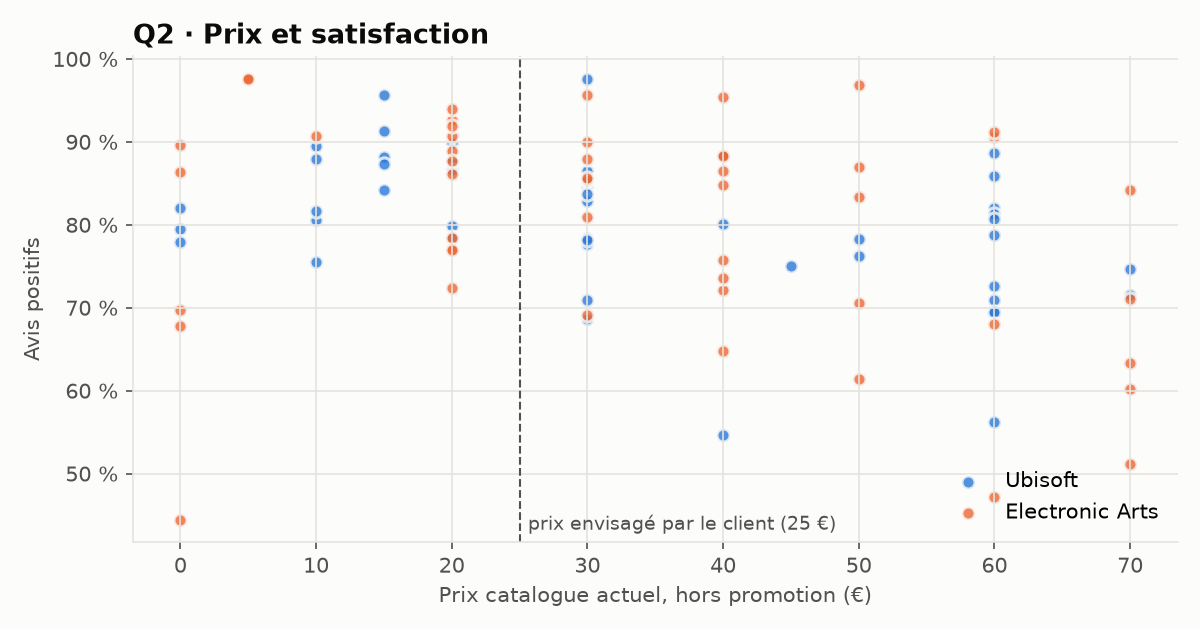
\includegraphics[width=0.88\linewidth]{q2_prix_satisfaction.png}
\caption{Prix catalogue actuel et satisfaction}
\end{figure}

Non, c'est plutôt l'inverse : la corrélation vaut $-0{,}55$ chez EA et $-0{,}46$ chez Ubisoft (Spearman : $-0{,}49$ pour les deux).
À 60~€ et plus, la médiane tombe à 63~\% (EA) et 73~\% (Ubisoft). La tranche 20 à 40~€, celle du client, se situe entre 80 et 86~\%.
Le prix étant le prix catalogue \emph{actuel}, un \textbf{biais du survivant} est possible : les anciens jeux peu chers qui se vendent
encore sont souvent des classiques.

\subsection{Q3 · Quels jeux gardent leurs joueurs ?}
\begin{figure}[H]
\centering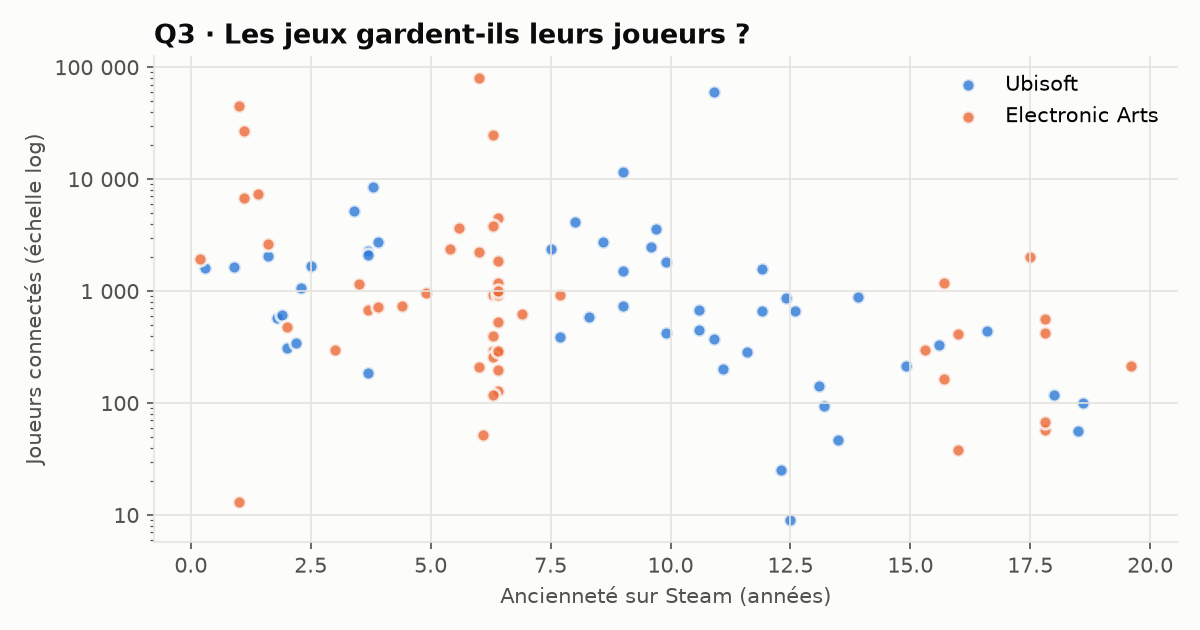
\includegraphics[width=0.88\linewidth]{q3_longevite.png}
\caption{Ancienneté sur Steam et joueurs connectés (échelle logarithmique)}
\end{figure}

Les quatre jeux de 5 ans et plus les plus joués sont \textbf{gratuits} : \textit{Apex Legends} (\num{79893} joueurs connectés),
\textit{Rainbow Six Siege} (\num{60193}), \textit{Les Sims 4} et \textit{Brawlhalla}. Parmi les jeux payants, ce sont le multijoueur,
la coopération (\textit{It Takes Two}, 95~\% d'avis positifs) et les grands jeux de rôle qui durent.

\subsection{Q4 · Les francophones jugent-ils différemment ?}
\begin{figure}[H]
\centering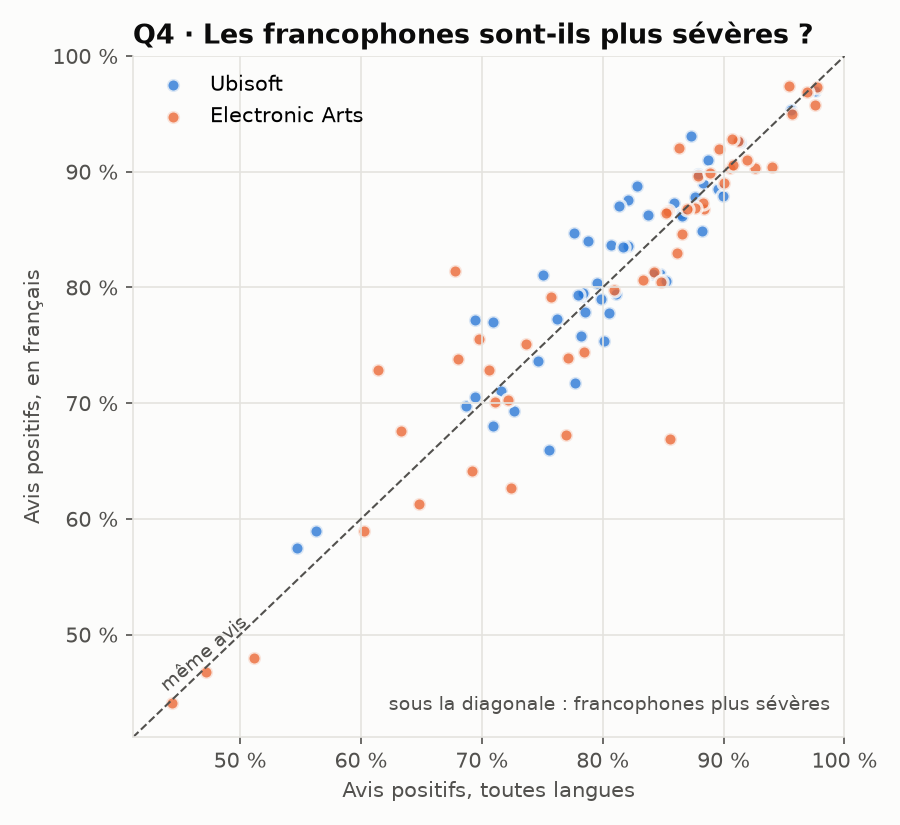
\includegraphics[width=0.6\linewidth]{q4_francophones.png}
\caption{Satisfaction en français et toutes langues, par jeu}
\end{figure}

Les francophones sont légèrement plus généreux, de +2,5 points envers EA et +2,1 envers Ubisoft. Sur 9 jeux Ubisoft ils sont nettement
plus positifs, contre 2 où ils sont plus sévères. Mais ils ne rédigent que \textbf{2~\% des avis}.

\subsection{Recommandations au client}
\begin{keybox}[Pour Lumen Forge Games]
\begin{enumerate}[leftmargin=1.4em]
  \item \textbf{Prix :} 25~€ se situe dans une tranche bien notée. Monter en prix, c'est monter les attentes.
  \item \textbf{Le lancement n'est pas un verdict :} prévoyez un calendrier de correctifs. Une réputation se redresse.
  \item \textbf{Surveillez les avis mois par mois :} une crise peut survenir des années après la sortie.
  \item \textbf{Durée de vie :} des mises à jour de contenu ou un mode coopératif prolongent la vie d'un jeu.
  \item \textbf{Marché :} traduisez le jeu en français, mais visez l'international, qui fait la réputation Steam.
\end{enumerate}
\end{keybox}

% =============================================================================
\section{Limites et dette technique}\label{sec:limites}

\begin{tabularx}{\linewidth}{@{}L{5.2cm} Y@{}}
\toprule
\textbf{Limite} & \textbf{Conséquence} \\
\midrule
Steam uniquement & Les conclusions portent sur les joueurs Steam, sans les autres plateformes \\
Instantané (mercredi, vers 19~h) & Pas de saisonnalité. Promotions non mesurables. \\
Prix catalogue actuel & Biais du survivant possible (Q2) \\
Ancienneté sur Steam & Différente de l'ancienneté réelle pour les jeux réédités (Q1b, Q3) \\
« Francophones » = avis en français & Ni le pays ni la langue maternelle ne sont connus \\
Corrélation & Elle ne prouve pas de causalité \\
\midrule
\multicolumn{2}{@{}l}{\textbf{Dette technique assumée au niveau 0}} \\
\midrule
Pas de tests unitaires & Introduits au projet 1 (\texttt{pytest}) \\
Pas de planification & Exécution manuelle. Orchestration prévue au projet 3. \\
Découverte non déterministe & Réserve R1. Parcourir tout le catalogue de l'éditeur. \\
Rechargement complet & Pas d'historique entre deux exécutions. Chargement incrémental prévu au projet 2. \\
\bottomrule
\end{tabularx}

% =============================================================================
\section{Retour d'expérience}
\begin{itemize}[leftmargin=1.2em]
  \item \textbf{Cadrer avant de coder :} une demande floue est devenue quatre questions mesurables, chacune liée à une décision du client.
  \item \textbf{Tester les API avant de promettre :} le paramètre \texttt{day\_range} ne fait pas ce que son nom suggère.
  \item \textbf{Se méfier des résultats parfaits :} « 0 exclusion » cachait un défaut de traçabilité.
  \item \textbf{Concevoir pour l'incident :} grâce au cache, une interruption s'est réglée en une minute.
  \item \textbf{Dire ce que les données ne permettent pas de conclure :} la question des promotions reste ouverte, et le rapport le dit.
\end{itemize}

% =============================================================================
\section{Feuille de route}
\begin{tabularx}{\linewidth}{@{}L{4.3cm} Y@{}}
\toprule
\textbf{Évolution} & \textbf{Apport} \\
\midrule
Tests et PostgreSQL & Robustesse et base serveur (projet 1 du portfolio) \\
Chargement incrémental quotidien & Historique des prix, saisonnalité, promotions (projet 2) \\
Orchestration et dbt & Planification, couches \emph{bronze, silver, gold} (projet 3) \\
Alerte de réputation & Notification quand la part d'avis positifs d'un mois passe sous un seuil \\
Panel d'éditeurs indépendants & Comparaison plus proche de la taille du client \\
\bottomrule
\end{tabularx}

% =============================================================================
\appendix
\section{Dictionnaire de données : table \texttt{games}}\label{ann:dico}
\small
\begin{longtable}{@{}L{4.1cm} L{2.0cm} L{8.3cm}@{}}
\toprule
\textbf{Colonne} & \textbf{Type} & \textbf{Description} \\
\midrule\endhead
\texttt{app\_id} & INTEGER & Identifiant Steam du jeu (clé primaire) \\
\texttt{name} & VARCHAR & Nom du jeu \\
\texttt{publisher\_group} & VARCHAR & Éditeur analysé : Ubisoft ou Electronic Arts \\
\texttt{publishers} / \texttt{developers} & VARCHAR & Éditeur(s) et studio(s) déclarés sur Steam \\
\texttt{is\_free} & BOOLEAN & Jeu gratuit (\emph{free-to-play}) \\
\texttt{price\_initial\_eur} & DECIMAL & Prix catalogue actuel hors promotion, en euros (et non le prix de lancement) \\
\texttt{price\_final\_eur} & DECIMAL & Prix payé le jour de l'extraction \\
\texttt{discount\_percent} & INTEGER & Remise en cours (\%) \\
\texttt{steam\_release\_date} & DATE & Date de sortie sur Steam \\
\texttt{years\_on\_steam} & DECIMAL & Ancienneté sur Steam au jour de l'extraction \\
\texttt{genres} & VARCHAR & Genres Steam, en français \\
\texttt{metacritic\_score} & INTEGER & Note de la presse, si disponible \\
\texttt{owners\_estimate\_low/high} & BIGINT & Fourchette SteamSpy du nombre de possesseurs \\
\texttt{extracted\_on} & DATE & Date de l'extraction \\
\bottomrule
\end{longtable}
\normalsize
Dictionnaire complet des cinq tables : \texttt{docs/dictionnaire-de-donnees.md}.

\section{Décisions d'architecture (ADR)}
\begin{tabularx}{\linewidth}{@{}l Y@{}}
\toprule
ADR 001 & Stack technique : DuckDB, pandas, \texttt{requests}, rechargement complet \\
ADR 002 & Stratégie d'extraction : deux passes, couche brute datée, cache, minimisation à la source \\
ADR 003 & Source de fréquentation : API officielle de Steam plutôt que SteamSpy \\
\bottomrule
\end{tabularx}

\section{Structure du dépôt}
\begin{lstlisting}[basicstyle=\ttfamily\footnotesize]
ubisoft-vs-ea-steam-etl/
|-- src/          extract.py, transform.py, load.py, report.py, pipeline.py, config.py
|-- sql/          00_schema.sql, q1a ... q4b (10 requetes), controle_recette.sql
|-- docs/
|   |-- mission/      brief, compte rendu de cadrage, cahier des charges
|   |-- decisions/    ADR 001 a 003
|   |-- journal/      journal de bord date
|   |-- livraison/    rapports PDF, resultats.md, figures, PV de recette
|   `-- rapport/      sources LaTeX de ce rapport
|-- data/         lots bruts et base DuckDB (non versionnes, regeneres par le pipeline)
|-- README.md  CHANGELOG.md  LICENSE  requirements.txt
\end{lstlisting}

\section{Glossaire}
\begin{tabularx}{\linewidth}{@{}>{\bfseries}L{3.6cm} Y@{}}
ETL & \emph{Extract, Transform, Load} : extraire, transformer, charger \\
Couche brute & Données conservées telles que reçues des sources, sans modification \\
Idempotence & Propriété d'un traitement qui donne le même résultat, qu'on l'exécute une ou plusieurs fois \\
Rechargement complet & Remplacement intégral des tables à chaque exécution (\emph{full refresh}) \\
Écriture atomique & Écriture qui réussit entièrement ou pas du tout \\
ADR & \emph{Architecture Decision Record} : fiche qui trace une décision technique et ses raisons \\
Recette & Vérification formelle, par le client, que le livrable respecte les critères convenus \\
\emph{Review bombing} & Afflux massif et soudain d'avis négatifs, souvent en réaction à une décision de l'éditeur \\
\end{tabularx}

\end{document}
